\section{Internal boundary conditions for MGM correction step}

%\subsection{Zero boundary ("BC-0")} 

%\[  \HL{I}{1}{n} = \HL{I}{2}{n} = 0 \]
Below, I will list three different ways to define Dirichlet boundary values for $\HS$ along mesh interfaces.
To this end, let me introduce the following notation for the mean value of $\HS$ in a given node $I$  
at interface $\partial M$ in time step $t_n$, which is only related to the x-direction and the 2-mesh case in Figure (3) of your summary,
\begin{equation}
\label{BC-MEAN}
\HLO{I}{n}:=  \frac{1}{2} \left[  \HL{IBAR}{1}{n}  +  \HL{1}{2}{n} \right] 
\end{equation}


\subsection{Simple mean value (SM)} 
In your section '(6.1) A simple solution'  you proposed to use the mean values of the $\HS$ values  from the last time step $t_{n-1}$
along the interface $\partial M$

\begin{equation}
\label{BC-SM}
\HL{I}{1}{n} = \HL{I}{2}{n} = \HLO{I}{n-1}  
\end{equation}

\subsection{Linear Extrapolation (LE)}

Due to my opinion another possible approach which probably gives a little more accuracy could be to use the mean values 
$\HLO{I}{n-1}$ and $\HLO{I}{n-2}$ of the two preceding time steps $t_{n-1}$ and $t_{n-2}$
and use linear extrapolation of these two values in time 
\begin{equation}
\label{BC-LE}
\HL{I}{1}{n} = \HL{I}{2}{n} =  2 \,\HLO{I}{n-1} - \, \HLO{I}{n-2}
\end{equation}
  
Of course it is the question of initial values for this extrapolation. I started with it only after the 2nd time-step and took (SM) before. 
But also for (SM) there is the question of the proper initial values from my point of view. Currently, I simply use zero as initial values $\HS$ values for $t_0$. However, I could also imagine to take a little more effort here (but more about this later).

\subsection{Taylor Series (TS)}

Now, let's come to your '(6.2) Complex solution' based on a Taylor series expansion.
\begin{align}
\HL{IBAR}{1}{n}  & =  \HL{I}{1}{n} - \frac{1}{1!}\frac{\DX}{2} \frac{\HPN{1}} {\DXP} \bigg|_{I}^n 
                                                    + \frac{1}{2!}\left(\frac{\DX}{2}\right)^2 \frac{\HPNT{1}} {\DXPT} \bigg|_{I}^n  - \cdots \label{BC-TSA}
 \\[1ex]
\HL{1}{2}{n}  & =  \HL{I}{2}{n} + \frac{1}{1!}\frac{\DX}{2} \frac{\HPN{2}} {\DXP} \bigg|_{I}^n 
                                                    + \frac{1}{2!}\left(\frac{\DX}{2}\right)^2 \frac{\HPNT{2}} {\DXPT} \bigg|_{I}^n  + \cdots   \nonumber                                                         
\end{align}
or shorter
\begin{align}
\HL{IBAR}{1}{n}  & =  \HL{I}{1}{n} - \frac{\DX}{2} \frac{\HPN{1}} {\DXP} \bigg|_{I}^n 
                                                     + \frac{\DXT}{\color{red}{8}} \frac{\HPNT{1}} {\DXPT} \bigg|_{I}^n  - \cdots \label{BC-TSB}
 \\[1ex]
\HL{1}{2}{n}  & =  \HL{I}{2}{n} + \frac{\DX}{2} \frac{\HPN{2}} {\DXP} \bigg|_{I}^n 
                                                     + \frac{\DXT}{\color{red}{8}}\frac{\HPNT{2}} {\DXPT} \bigg|_{I}^n  + \cdots    \nonumber                                                 
\end{align}



%Please have a look at the '8' in the denominator where you had a '4'. But we still have to divide the $(\DX / 2)^2$ term by '$2!$'. Isn't that correct? 
For the ghost cell values $\HL{IBAR+1}{1}{n}$ and $\HL{0}{2}{n}$ we consider linear extrapolation
\begin{align}
\label{Extrapolation}
\HL{{\color{red}{IBAR+1}}}{1}{n} & = 2\, \HL{{\color{green}{I}}}{1}{n} -  \HL{{\color{red}{IBAR}}}{1}{n} \\[1ex]
\HL{{\color{blue}{0}}}{2}{n} & = 2 \,\HL{{\color{green}{I}}}{2}{n} -  \HL{{\color{blue}{1}}}{2}{n}   \nonumber     
\end{align}

\begin{figure}[H]
\begin{center}
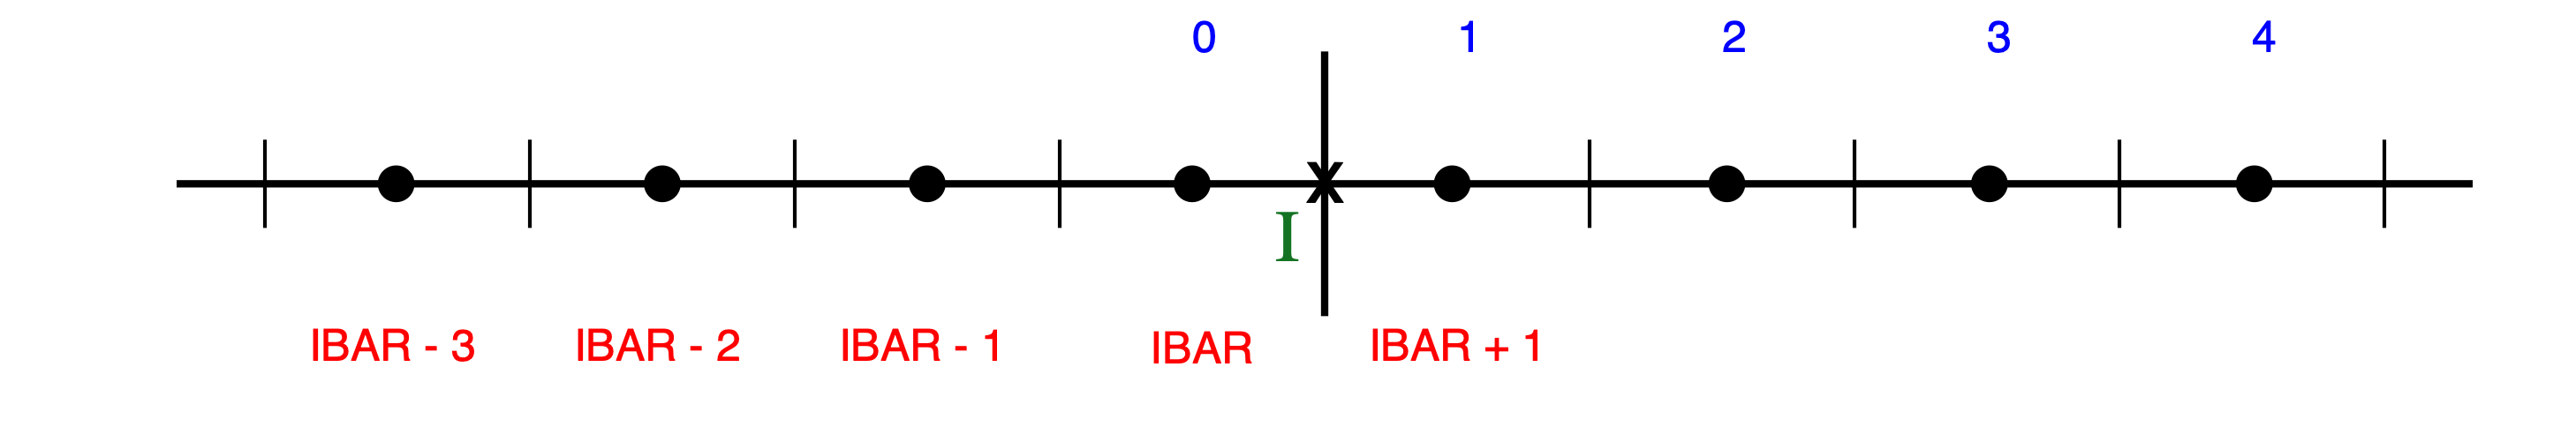
\includegraphics[width=14cm]{\figPath/DecompositionX.png}
\end{center}
\caption{Decomposition in x-direction}
\label{FIG_DecompositionX}
\end{figure}
In the following I will list the individual steps in great detail to avoid sign errors or similar in a possible implementation. 
First of all the following simple transformation is done based on (\ref{BC-TSB})


\begin{align}
\label{BC-TSB}
\HL{I}{1}{n} & = \HL{IBAR}{1}{n}  + \frac{\DX}{2} \frac{\HPN{1}} {\DXP} \bigg|_{I}^n 
                                                      - \frac{\DXT}{8} \frac{\HPNT{1}} {\DXPT} \bigg|_{I}^n  + \cdots  \\[1ex]
\HL{I}{2}{n} & =  \HL{1}{2}{n}  - \frac{\DX}{2} \frac{\HPN{2}} {\DXP} \bigg|_{I}^n 
                                                - \frac{\DXT}{8}\frac{\HPNT{2}} {\DXPT} \bigg|_{I}^n  - \cdots         \nonumber                                            
\end{align}


Now, substituting the interface values (\ref{BC-TSB}) into the extrapolation settings (\ref{Extrapolation}) in order to eliminate them
\begin{align}
\HL{IBAR+1}{1}{n} & \; \approx 2 \cdot \left( \HL{IBAR}{1}{n}  + \frac{\DX}{2} \frac{\HPN{1}} {\DXP} \bigg|_{I}^n 
                                                      - \frac{\DXT}{8} \frac{\HPNT{1}} {\DXPT} \bigg|_{I}^n  \right) -  \HL{IBAR}{1}{n} \label{BC-TSDA}
 \\[1ex]
\HL{0}{2}{n} & \approx \; 2 \cdot \left( \HL{1}{2}{n}  - \frac{\DX}{2} \frac{\HPN{2}} {\DXP} \bigg|_{I}^n 
                                                - \frac{\DXT}{8}\frac{\HPNT{2}} {\DXPT} \bigg|_{I}^n \right)    -  \HL{1}{2}{n}      \nonumber                                           
\end{align}
which finally leads to

\begin{align}
\HL{IBAR+1}{1}{n} & \approx \;  \HL{IBAR}{1}{n}  + \DX \frac{\HPN{1}} {\DXP} \bigg|_{I}^n 
                                                      - \frac{\DXT}{4} \frac{\HPNT{1}} {\DXPT} \bigg|_{I}^n  \label{BC-TSDB}
 \\[1ex]
\HL{0}{2}{n} & \approx  \HL{1}{2}{n}  - \DX \frac{\HPN{2}} {\DXP} \bigg|_{I}^n 
                                                - \frac{\DXT}{4}\frac{\HPNT{2}} {\DXPT} \bigg|_{I}^n     \nonumber                                           
\end{align}

\newpage
\subsubsection{The second derivative}
As you wrote, the second derivative in x must be the negative of the second derivative in y, because we solve the Laplace problem.
%\[ \frac{\HPNT{1}}{\DXPT} \bigg|_{I}^n  = -  \frac{\HPNT{1}}{\DYPT}\bigg|_{I}^n   \]

But concerning your second step in the derivation under '(6.3) Second derivative' I am confused right now. There you use two terms, first a difference quotient in y and then one in x (but our goal is to replace '$IBAR+1$'). Here, I suppose we only need the first one in y such that finally holds
\begin{align}
\label{BC-TSE}
 \frac{\HPNT{1}}{\DXPT} \bigg|_{I}^n  & = -  \frac{\HPNT{1}}{\DYPT}\bigg|_{I}^n   \approx 
                                                                  - \,\frac{\HL{IBAR,j-1}{1}{n} - 2 \HL{IBAR,j}{1}{n} + \HL{IBAR,j+1}{1}{n}}{\DYT}        \\                                                                 
 \frac{\HPNT{2}}{\DXPT} \bigg|_{I}^n  & = -  \frac{\HPNT{2}}{\DYPT}\bigg|_{I}^n   \approx 
                                                                  - \, \frac{\HL{1,j-1}{2}{n} - 2 \HL{1,j}{2}{n} + \HL{1,j+1}{2}{n}}{\DYT} 
\end{align}                                                                  

What do you think about this? This term adds matrix entries in y-direction.

\subsubsection{The first derivative}
For the sake of completeness I also list your steps to define the first derivation. Based on the previous solutions
$\HL{\,}{1}{n-1}$ and $\HL{\,}{2}{n-1}$, we approximate the derivative on the mesh interface by

\[ \frac {\HPNT{1}}{\DXP}\bigg|_{I}^n  = \frac {\HPNT{2}}{\DXP}\bigg|_{I}^n \approx \frac{\HL{1}{2}{n-1} - \HL{IBAR}{1}{n-1}} {\DX}\]

\subsubsection{Putting everything together}

Now, inserting all this stuff into (\ref{BC-TSD}) we get
\begin{align}
\label{BC-TSF}
\HL{IBAR+1,j}{1}{n} & \approx \;  \HL{IBAR,j}{1}{n}  + \DX \left( \frac{\HL{1}{2}{n-1} - \HL{IBAR,j}{1}{n-1}} {\DX}\right)
                                                      - \frac{\DXT}{4}   \left(-\,\frac{\HL{IBAR,j-1}{1}{n} - 2 \HL{IBAR,j}{1}{n} + \HL{IBAR,j+1}{1}{n}}{\DYT} \right)
 \\[1ex]
\HL{0,j}{2}{n} & \approx  \HL{1,j}{2}{n}  - \DX \left(\frac{\HL{1,j}{2}{n-1} - \HL{IBAR,j}{1}{n-1}} {\DX}\right)
                                                - \frac{\DXT}{4} \left(-\,\frac{\HL{1,j-1}{2}{n} - 2 \HL{1,j}{2}{n} + \HL{1,j+1}{2}{n}}{\DYT}  \right)    \nonumber                                           
\end{align}

And if I didn't make a mistake somewhere (which is not unlikely in this mess), this finally leads to
\begin{align}
\label{BC-TSF}
\HL{IBAR+1,j}{1}{n} & \approx \;  \HL{IBAR,j}{1}{n}  + \left(\HL{1,j}{2}{n-1} - \HL{IBAR,j}{1}{n-1}\right) 
                                                + \frac{\DXT}{4\DYT}   \left(\HL{IBAR,j-1}{1}{n} - 2 \HL{IBAR,j}{1}{n} + \HL{IBAR,j+1}{1}{n} \right) \\[1ex]
\HL{0,j}{2}{n} & \approx  \HL{1,j}{2}{n}  - \left( \HL{1,j}{2}{n-1} - \HL{IBAR,j}{1}{n-1}\right)
                                                + \frac{\DXT}{4\DYT}   \left(\HL{1,j-1}{2}{n} - 2 \HL{1,j}{2}{n} + \HL{1,j+1}{2}{n}\right)      \nonumber                                           
\end{align}
When using these terms in the matrix stencil for cells adjacent to the mesh interface, the previous '${n-1}$' terms add up to the right hand side and the current '$n$' terms to the matrix itself.

\subsubsection{Substituting the ghost values in the matrix stencil in 2D}
%
\paragraph{Mesh 1:} 
For a cell in mesh 1 adjacent to the mesh interface the usual Laplace matrix stencil is
\[   \frac{ \HL{IBAR-1,j}{1}{n} -2 \HL{IBAR,j}{1}{n} + \HL{IBAR+1,j}{1}{n} }{\DXT} +  
    \frac{ \HL{IBAR,j-1}{1}{n} -2 \HL{IBAR,j}{1}{n} + \HL{IBAR,j+1}{1}{n} }{\DYT} = 0 \]
Now, substituting the '$IBAR+1$' component based on the derivation in (\ref{BC-TSF}), we get 
\[ {\scriptstyle  \frac{ \HL{IBAR-1,j}{1}{n} -2 \HL{IBAR,j}{1}{n} 
+ \left[ \HL{IBAR,j}{1}{n}  + \left(\HL{1,j}{2}{n-1} - \HL{IBAR,j}{1}{n-1}\right) + \frac{\DXT}{4\DYT}   \left(\HL{IBAR,j-1}{1}{n} - 2 \HL{IBAR,j}{1}{n} + \HL{IBAR,j+1}{1}{n} \right) \right]}{\DXT}
+      \frac{ \HL{IBAR,j-1}{1}{n} -2 \HL{IBAR,j}{1}{n} + \HL{IBAR,j+1}{1}{n} }{\DYT} = 0}
\]
Let's first move the previous '${n-1}$' terms on the right hand side and sum up the obvious
\[ {\scriptstyle  \frac{ \HL{IBAR-1,j}{1}{n} - \HL{IBAR,j}{1}{n}   
+ \frac{\DXT}{4\DYT}   \left(\HL{IBAR,j-1}{1}{n} - 2 \HL{IBAR,j}{1}{n} + \HL{IBAR,j+1}{1}{n} \right) }{\DXT}
+      \frac{ \HL{IBAR,j-1}{1}{n} -2 \HL{IBAR,j}{1}{n} + \HL{IBAR,j+1}{1}{n} }{\DYT} = -\frac{\HL{1,j}{2}{n-1} - \HL{IBAR,j}{1}{n-1}}{\DXT} }
\]
and then resort the whole stuff
\[ {\scriptstyle 
      \HL{IBAR,j-1}{1}{n} \left( \frac {1}{4\DYT} + \frac {1}{\DYT}    \right)
 +   \HL{IBAR-1,j}{1}{n} \left( \frac {1}{\DXT} \right)
 +   \HL{IBAR,j}{1}{n} \left( -\frac {1}{\DXT} - \frac {1}{2\DYT} - \frac {2}{\DYT}    \right)
 +   \HL{IBAR,j+1}{1}{n} \left( \frac {1}{4\DYT}   + \frac {1}{\DYT}    \right)
    = -\frac{\HL{1,j}{2}{n-1} - \HL{IBAR,j}{1}{n-1}}{\DXT} }
\]
which finally gives the new matrix entries for the corresponding matrix line for cell $(IBAR,j)$ in mesh 1. 

%\HL{2,j}{2}{n}
\paragraph{Mesh 2:} 

\vspace{0.5cm}
For a cell in mesh 2 adjacent to the mesh interface the usual Laplace matrix stencil is
\[   
   \frac{ \HL{0,j}{2}{n} -2 \HL{1,j}{2}{n} + \HL{2,j}{2}{n} }{\DXT} +  
   \frac{ \HL{1,j-1}{2}{n} -2 \HL{1,j}{2}{n} + \HL{1,j+1}{2}{n} }{\DYT} = 0 
\]
Now, substituting the '$0$' component based on the derivation in (\ref{BC-TSF}), we get 
\[ 
  {\scriptstyle  
   \frac{ 
   \left[
         \HL{1,j}{2}{n}  - \left( \HL{1,j}{2}{n-1} - \HL{IBAR,j}{1}{n-1}\right)
      + \frac{\DXT}{4\DYT}   \left(\HL{1,j-1}{2}{n} - 2 \HL{1,j}{2}{n} + \HL{1,j+1}{2}{n}\right)
   \right] 
   -2 \HL{1,j}{2}{n} + \HL{2,j}{2}{n} }{\DXT} +  
   \frac{ \HL{1,j-1}{2}{n} -2 \HL{1,j}{2}{n} + \HL{1,j+1}{2}{n} }{\DYT} = 0 
   }
\]
Let's first move the previous '${n-1}$' terms on the right hand side and sum up the obvious
\[ 
  {\scriptstyle  
   \frac{ 
         -\HL{1,j}{2}{n}  
      + \frac{\DXT}{4\DYT}   \left(\HL{1,j-1}{2}{n} - 2 \HL{1,j}{2}{n} + \HL{1,j+1}{2}{n}\right)
 + \HL{2,j}{2}{n} }{\DXT} +  
   \frac{ \HL{1,j-1}{2}{n} -2 \HL{1,j}{2}{n} + \HL{1,j+1}{2}{n} }{\DYT} =  \frac{\HL{1,j}{2}{n-1} - \HL{IBAR,j}{1}{n-1}}{\DXT}
   }
\]


and then resort the whole stuff
\[ {\scriptstyle 
      \HL{1,j-1}{2}{n} \left( \frac {1}{4\DYT} + \frac {1}{\DYT}    \right)
 +   \HL{2,j}{2}{n} \left( \frac {1}{\DXT} \right)
 +   \HL{1,j}{2}{n} \left( -\frac {1}{\DXT} - \frac {1}{2\DYT} - \frac {2}{\DYT}    \right)
 +    \HL{1,j+1}{2}{n} \left( \frac {1}{4\DYT}   + \frac {1}{\DYT}    \right)
    = \frac{\HL{1,j}{2}{n-1} - \HL{1,j}{1}{n-1}}{\DXT} }
\]
which finally gives the new matrix entries for the corresponding matrix line for cell $(1,j)$ in mesh 2.

\newpage

\subsubsection{Substituting the ghost values in the matrix stencil in 3D}
%
\paragraph{Mesh 1:} 
For a cell in mesh 1 adjacent to the mesh interface the usual Laplace matrix stencil is
\begin{align}   
    & \frac{ \HL{IBAR-1,j,k}{1}{n} -2 \HL{IBAR,j,k}{1}{n} + \HL{IBAR+1,j,k}{1}{n} }{\DXT} \\
+  & \frac{ \HL{IBAR,j-1,k}{1}{n} -2 \HL{IBAR,j,k}{1}{n} + \HL{IBAR,j+1,k}{1}{n} }{\DYT} \\
+  & \frac{ \HL{IBAR,j-1,k}{1}{n} -2 \HL{IBAR,j,k}{1}{n} + \HL{IBAR,j+1,k}{1}{n} }{\DYT} \\
& \hspace{5cm}= 0 
 \end{align}
Now, substituting the '$IBAR+1$' component based on the derivation in (\ref{BC-TSF}), we get 
\[ {\scriptstyle  \frac{ \HL{IBAR-1,j}{1}{n} -2 \HL{IBAR,j}{1}{n} 
+ \left[ \HL{IBAR,j}{1}{n}  + \left(\HL{1,j}{2}{n-1} - \HL{IBAR,j}{1}{n-1}\right) + \frac{\DXT}{4\DYT}   \left(\HL{IBAR,j-1}{1}{n} - 2 \HL{IBAR,j}{1}{n} + \HL{IBAR,j+1}{1}{n} \right) \right]}{\DXT}
+      \frac{ \HL{IBAR,j-1}{1}{n} -2 \HL{IBAR,j}{1}{n} + \HL{IBAR,j+1}{1}{n} }{\DYT} = 0}
\]
Let's first move the previous '${n-1}$' terms on the right hand side and sum up the obvious
\[ {\scriptstyle  \frac{ \HL{IBAR-1,j}{1}{n} - \HL{IBAR,j}{1}{n}   
+ \frac{\DXT}{4\DYT}   \left(\HL{IBAR,j-1}{1}{n} - 2 \HL{IBAR,j}{1}{n} + \HL{IBAR,j+1}{1}{n} \right) }{\DXT}
+      \frac{ \HL{IBAR,j-1}{1}{n} -2 \HL{IBAR,j}{1}{n} + \HL{IBAR,j+1}{1}{n} }{\DYT} = -\frac{\HL{1,j}{2}{n-1} - \HL{IBAR,j}{1}{n-1}}{\DXT} }
\]
and then resort the whole stuff
\[ {\scriptstyle 
      \HL{IBAR,j-1}{1}{n} \left( \frac {1}{4\DYT} + \frac {1}{\DYT}    \right)
 +   \HL{IBAR-1,j}{1}{n} \left( \frac {1}{\DXT} \right)
 +   \HL{IBAR,j}{1}{n} \left( -\frac {1}{\DXT} - \frac {1}{2\DYT} - \frac {2}{\DYT}    \right)
 +   \HL{IBAR,j+1}{1}{n} \left( \frac {1}{4\DYT}   + \frac {1}{\DYT}    \right)
    = -\frac{\HL{1,j}{2}{n-1} - \HL{IBAR,j}{1}{n-1}}{\DXT} }
\]
which finally gives the new matrix entries for the corresponding matrix line for cell $(IBAR,j)$ in mesh 1. 


This is all done in extreme detail now, but I found it more secure than on paper, thanks to Copy\&Paste. I really hope that not one million sign and component errors have crept in here. I'll focus on the code again now.

Have I understood your suggested procedure correctly by then or do you think that the above derivations are correct so far?

